%\documentclass[11pt,a4paper,titlepage,twoside]{article}
\documentclass[12pt,a4paper,twoside]{article}
%\documentclass[12pt,a4paper,twoside]{scrartcl}
\usepackage{mystyle}
\usepackage{gplot}
\usepackage{mechanik_v001}
\usepackage{foto_v001}


\usepackage[shell]{gnuplottex}
\usepackage{pgf}
\usepackage{pgfplots}
\usepackage{gnuplot-lua-tikz}
\pgfplotsset{compat=1.9}




%\author{Felix Binder}
\title{Wärmelehre}
\date{}



\def\dir{./Aufgaben_Waerme/}
\newcommand{\Einbinden}[1]{\input{#1}}


\begin{document}
\maketitle

%Aufgabe
%Bauen Sie einen Heissluftballon.


%Skizzieren Sie den Aufbau

\section*{Temperatur}

\Einbinden{\dir/lueckentext_temperatur.tex}
\newpage

\section*{Atomtheorie der Materie}
\Einbinden{\dir/lueckentext_atomtheorie01.tex}




\section*{Innere Energie}
\Einbinden{\dir/lueckentext_innereenergie.tex}

\newpage

%Auf dem Pult stehen drei Schalen mit Wasser. Jede hat eine andere Temperatur.
%Halten Sie eine Hand in das kalte Wasser und eine ins lauwarme Wasser. Was spüren Sie?
%muss ich noch ausbauen

%\section*{Messung der Temperatur}
%Für technische und physikalische Fragestellungen braucht man eine Möglichkeit die Temperatur
%reproduzierbar und in einem grossen Spektrum zu messen. Die Sinneszellen der Haut können diese Aufgabe nicht erfüllen.
%Um die Temperatur technisch zu messen werden Thermometer benutzt.



%\section*{Thermische Ausdehnung}
%\subsection*{Feste Körper}
%\subsection*{Gase}
\section*{Das ideale Gas}
Das ideale Gas ist ein Modellsystem das eingeführt wird, um das verhalten von Gasen zu erklären.
Viele reale Gase verhalten sich bei niedrigen Drücken wie das ideale Gas.
Eigenschaften des idealen Gases sind:
\begin{itemize}
	\item Das ideale Gas besteht aus punktförmigen ``Atomen'' ohne Volumen.
	\item Die ``Atome'' des idealen Gases Wechselwirken nicht miteinander. 
		Das heisst es gibt weder Anziehung noch Abstossung zwischen den ``Atomen''.
	\item Die ``Atome'' sind ständig in Bewegung. Wenn sie mit der begrenzenden Gefässwand kollidieren, 
		geschieht dies ohne Energieverlust.
\end{itemize}

Im folgenden wollen wir die Eigenschaften des idealen Gases untersuchen.

\subsection*{Zusammenhang von Druck und Temperatur beim idealen Gas}
In einem Experiment wird ein verdünntes Gas in einem Glaskolben erwärmt.
Für einige festgelegte Temperaturen wird der Druck des Gases gemessen.
In einem zweiten Durchgang des Experiments wird die Gasmenge leicht erhöht.
Das Volumen und die Gasmenge sind während des gesamten Experiments konstant.
In der nachfolgenden Tabelle sind Temperatur und Druck für die zwei Durchgänge des Experiments angegeben.

\begin{center}
\begin{tabular}{lcccccc}
Temperatur &		\SI{0}{\celsius} & \SI{20}{\celsius} & \SI{40}{\celsius} & \SI{60}{\celsius} & \SI{80}{\celsius} & \SI{100}{\celsius}\\
Durchgang 1 &  \SI{100.2}{hPa}         & \SI{106.6}{hPa}   & \SI{114.7}{hPa}   & \SI{122.3}{hPa}   & \SI{130.0}{hPa}   & \SI{136.3}{hPa}\\
Durchgang 2 &  \SI{149.9}{hPa}	     & \SI{161.0}{hPa}   & \SI{172.5}{hPa}   & \SI{182.4}{hPa}   & \SI{194.0}{hPa}   & \SI{205.5}{hPa}\\
\end{tabular}
\end{center}

\begin{aufgabe}
\begin{itemize}
\item Zeichnen Sie die Messwerte aus der Tabelle in ein $Tp$-Diagramm ein.
\item Beschreiben Sie wie sich der Druck in Abhängigkeit zur Temperatur verändert.
\item Was passiert, wenn Sie die Messwerte des Diagramms auf den Druck von \SI{0}{hPa} extrapolieren?
\end{itemize}
\begin{loesung}
	\begin{itemize}
		\item [a)] Hier das $p$-$T$-Diagramm.\par
	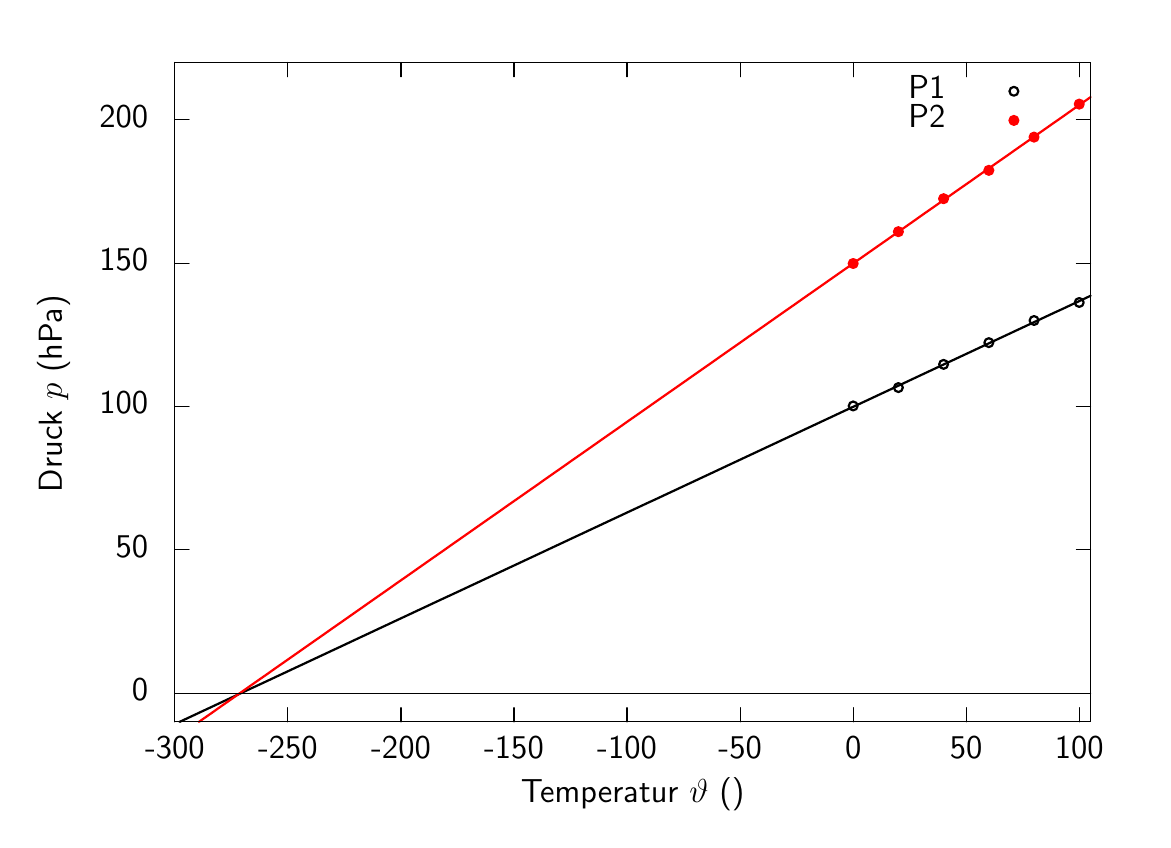
\begin{tikzpicture}[gnuplot]
%% generated with GNUPLOT 4.6p1 (Lua 5.1; terminal rev. 99, script rev. 100)
%% Mit 01 Mai 2013 11:47:56 CEST
\tikzset{every node/.append style={font={\sffamily\fontsize{12pt}{14.4pt}\selectfont}}}
\path (0.000,0.000) rectangle (14.100,10.000);
\gpcolor{color=gp lt color border}
\gpsetlinetype{gp lt border}
\gpsetlinewidth{1.00}
\draw[gp path] (1.806,1.548)--(1.986,1.548);
\draw[gp path] (13.436,1.548)--(13.256,1.548);
\node[gp node right] at (1.585,1.548) { 0};
\draw[gp path] (1.806,3.368)--(1.986,3.368);
\draw[gp path] (13.436,3.368)--(13.256,3.368);
\node[gp node right] at (1.585,3.368) { 50};
\draw[gp path] (1.806,5.188)--(1.986,5.188);
\draw[gp path] (13.436,5.188)--(13.256,5.188);
\node[gp node right] at (1.585,5.188) { 100};
\draw[gp path] (1.806,7.009)--(1.986,7.009);
\draw[gp path] (13.436,7.009)--(13.256,7.009);
\node[gp node right] at (1.585,7.009) { 150};
\draw[gp path] (1.806,8.829)--(1.986,8.829);
\draw[gp path] (13.436,8.829)--(13.256,8.829);
\node[gp node right] at (1.585,8.829) { 200};
\draw[gp path] (1.806,1.184)--(1.806,1.364);
\draw[gp path] (1.806,9.557)--(1.806,9.377);
\node[gp node center] at (1.806,0.814) {-300};
\draw[gp path] (3.242,1.184)--(3.242,1.364);
\draw[gp path] (3.242,9.557)--(3.242,9.377);
\node[gp node center] at (3.242,0.814) {-250};
\draw[gp path] (4.678,1.184)--(4.678,1.364);
\draw[gp path] (4.678,9.557)--(4.678,9.377);
\node[gp node center] at (4.678,0.814) {-200};
\draw[gp path] (6.113,1.184)--(6.113,1.364);
\draw[gp path] (6.113,9.557)--(6.113,9.377);
\node[gp node center] at (6.113,0.814) {-150};
\draw[gp path] (7.549,1.184)--(7.549,1.364);
\draw[gp path] (7.549,9.557)--(7.549,9.377);
\node[gp node center] at (7.549,0.814) {-100};
\draw[gp path] (8.985,1.184)--(8.985,1.364);
\draw[gp path] (8.985,9.557)--(8.985,9.377);
\node[gp node center] at (8.985,0.814) {-50};
\draw[gp path] (10.421,1.184)--(10.421,1.364);
\draw[gp path] (10.421,9.557)--(10.421,9.377);
\node[gp node center] at (10.421,0.814) { 0};
\draw[gp path] (11.857,1.184)--(11.857,1.364);
\draw[gp path] (11.857,9.557)--(11.857,9.377);
\node[gp node center] at (11.857,0.814) { 50};
\draw[gp path] (13.292,1.184)--(13.292,1.364);
\draw[gp path] (13.292,9.557)--(13.292,9.377);
\node[gp node center] at (13.292,0.814) { 100};
\draw[gp path] (1.806,9.557)--(1.806,1.184)--(13.436,1.184)--(13.436,9.557)--cycle;
\node[gp node center,rotate=-270] at (0.295,5.370) {Druck $p$ (hPa)};
\node[gp node center] at (7.621,0.259) {Temperatur $\vartheta$ (\SI{}{\celsius})};
\node[gp node right] at (11.709,9.192) {P1};
\gpcolor{rgb color={0.000,0.000,0.000}}
\gpsetlinewidth{2.00}
\gpsetpointsize{4.00}
\gppoint{gp mark 6}{(10.421,5.196)}
\gppoint{gp mark 6}{(10.995,5.429)}
\gppoint{gp mark 6}{(11.569,5.724)}
\gppoint{gp mark 6}{(12.144,6.000)}
\gppoint{gp mark 6}{(12.718,6.281)}
\gppoint{gp mark 6}{(13.292,6.510)}
\gppoint{gp mark 6}{(12.462,9.192)}
\gpsetlinetype{gp lt plot 0}
\draw[gp path] (1.868,1.184)--(1.923,1.210)--(2.041,1.265)--(2.158,1.320)--(2.276,1.375)%
  --(2.393,1.430)--(2.511,1.485)--(2.628,1.540)--(2.746,1.595)--(2.863,1.649)--(2.981,1.704)%
  --(3.098,1.759)--(3.216,1.814)--(3.333,1.869)--(3.451,1.924)--(3.568,1.979)--(3.686,2.034)%
  --(3.803,2.089)--(3.921,2.144)--(4.038,2.199)--(4.155,2.254)--(4.273,2.309)--(4.390,2.364)%
  --(4.508,2.419)--(4.625,2.474)--(4.743,2.529)--(4.860,2.584)--(4.978,2.639)--(5.095,2.694)%
  --(5.213,2.749)--(5.330,2.803)--(5.448,2.858)--(5.565,2.913)--(5.683,2.968)--(5.800,3.023)%
  --(5.918,3.078)--(6.035,3.133)--(6.153,3.188)--(6.270,3.243)--(6.388,3.298)--(6.505,3.353)%
  --(6.622,3.408)--(6.740,3.463)--(6.857,3.518)--(6.975,3.573)--(7.092,3.628)--(7.210,3.683)%
  --(7.327,3.738)--(7.445,3.793)--(7.562,3.848)--(7.680,3.903)--(7.797,3.958)--(7.915,4.012)%
  --(8.032,4.067)--(8.150,4.122)--(8.267,4.177)--(8.385,4.232)--(8.502,4.287)--(8.620,4.342)%
  --(8.737,4.397)--(8.854,4.452)--(8.972,4.507)--(9.089,4.562)--(9.207,4.617)--(9.324,4.672)%
  --(9.442,4.727)--(9.559,4.782)--(9.677,4.837)--(9.794,4.892)--(9.912,4.947)--(10.029,5.002)%
  --(10.147,5.057)--(10.264,5.112)--(10.382,5.167)--(10.499,5.221)--(10.617,5.276)--(10.734,5.331)%
  --(10.852,5.386)--(10.969,5.441)--(11.087,5.496)--(11.204,5.551)--(11.321,5.606)--(11.439,5.661)%
  --(11.556,5.716)--(11.674,5.771)--(11.791,5.826)--(11.909,5.881)--(12.026,5.936)--(12.144,5.991)%
  --(12.261,6.046)--(12.379,6.101)--(12.496,6.156)--(12.614,6.211)--(12.731,6.266)--(12.849,6.321)%
  --(12.966,6.376)--(13.084,6.430)--(13.201,6.485)--(13.319,6.540)--(13.436,6.595);
\gpcolor{color=gp lt color border}
\node[gp node right] at (11.709,8.822) {P2};
\gpcolor{rgb color={1.000,0.000,0.000}}
\gppoint{gp mark 7}{(10.421,7.005)}
\gppoint{gp mark 7}{(10.995,7.409)}
\gppoint{gp mark 7}{(11.569,7.828)}
\gppoint{gp mark 7}{(12.144,8.188)}
\gppoint{gp mark 7}{(12.718,8.610)}
\gppoint{gp mark 7}{(13.292,9.029)}
\gppoint{gp mark 7}{(12.462,8.822)}
\draw[gp path] (2.113,1.184)--(2.158,1.216)--(2.276,1.298)--(2.393,1.381)--(2.511,1.463)%
  --(2.628,1.545)--(2.746,1.628)--(2.863,1.710)--(2.981,1.792)--(3.098,1.875)--(3.216,1.957)%
  --(3.333,2.039)--(3.451,2.122)--(3.568,2.204)--(3.686,2.286)--(3.803,2.369)--(3.921,2.451)%
  --(4.038,2.533)--(4.155,2.615)--(4.273,2.698)--(4.390,2.780)--(4.508,2.862)--(4.625,2.945)%
  --(4.743,3.027)--(4.860,3.109)--(4.978,3.192)--(5.095,3.274)--(5.213,3.356)--(5.330,3.439)%
  --(5.448,3.521)--(5.565,3.603)--(5.683,3.686)--(5.800,3.768)--(5.918,3.850)--(6.035,3.933)%
  --(6.153,4.015)--(6.270,4.097)--(6.388,4.179)--(6.505,4.262)--(6.622,4.344)--(6.740,4.426)%
  --(6.857,4.509)--(6.975,4.591)--(7.092,4.673)--(7.210,4.756)--(7.327,4.838)--(7.445,4.920)%
  --(7.562,5.003)--(7.680,5.085)--(7.797,5.167)--(7.915,5.250)--(8.032,5.332)--(8.150,5.414)%
  --(8.267,5.496)--(8.385,5.579)--(8.502,5.661)--(8.620,5.743)--(8.737,5.826)--(8.854,5.908)%
  --(8.972,5.990)--(9.089,6.073)--(9.207,6.155)--(9.324,6.237)--(9.442,6.320)--(9.559,6.402)%
  --(9.677,6.484)--(9.794,6.567)--(9.912,6.649)--(10.029,6.731)--(10.147,6.814)--(10.264,6.896)%
  --(10.382,6.978)--(10.499,7.060)--(10.617,7.143)--(10.734,7.225)--(10.852,7.307)--(10.969,7.390)%
  --(11.087,7.472)--(11.204,7.554)--(11.321,7.637)--(11.439,7.719)--(11.556,7.801)--(11.674,7.884)%
  --(11.791,7.966)--(11.909,8.048)--(12.026,8.131)--(12.144,8.213)--(12.261,8.295)--(12.379,8.377)%
  --(12.496,8.460)--(12.614,8.542)--(12.731,8.624)--(12.849,8.707)--(12.966,8.789)--(13.084,8.871)%
  --(13.201,8.954)--(13.319,9.036)--(13.436,9.118);
\gpcolor{color=gp lt color border}
\gpsetlinetype{gp lt border}
\gpsetlinewidth{1.00}
\draw[gp path] (1.806,1.548)--(1.923,1.548)--(2.041,1.548)--(2.158,1.548)--(2.276,1.548)%
  --(2.393,1.548)--(2.511,1.548)--(2.628,1.548)--(2.746,1.548)--(2.863,1.548)--(2.981,1.548)%
  --(3.098,1.548)--(3.216,1.548)--(3.333,1.548)--(3.451,1.548)--(3.568,1.548)--(3.686,1.548)%
  --(3.803,1.548)--(3.921,1.548)--(4.038,1.548)--(4.155,1.548)--(4.273,1.548)--(4.390,1.548)%
  --(4.508,1.548)--(4.625,1.548)--(4.743,1.548)--(4.860,1.548)--(4.978,1.548)--(5.095,1.548)%
  --(5.213,1.548)--(5.330,1.548)--(5.448,1.548)--(5.565,1.548)--(5.683,1.548)--(5.800,1.548)%
  --(5.918,1.548)--(6.035,1.548)--(6.153,1.548)--(6.270,1.548)--(6.388,1.548)--(6.505,1.548)%
  --(6.622,1.548)--(6.740,1.548)--(6.857,1.548)--(6.975,1.548)--(7.092,1.548)--(7.210,1.548)%
  --(7.327,1.548)--(7.445,1.548)--(7.562,1.548)--(7.680,1.548)--(7.797,1.548)--(7.915,1.548)%
  --(8.032,1.548)--(8.150,1.548)--(8.267,1.548)--(8.385,1.548)--(8.502,1.548)--(8.620,1.548)%
  --(8.737,1.548)--(8.854,1.548)--(8.972,1.548)--(9.089,1.548)--(9.207,1.548)--(9.324,1.548)%
  --(9.442,1.548)--(9.559,1.548)--(9.677,1.548)--(9.794,1.548)--(9.912,1.548)--(10.029,1.548)%
  --(10.147,1.548)--(10.264,1.548)--(10.382,1.548)--(10.499,1.548)--(10.617,1.548)--(10.734,1.548)%
  --(10.852,1.548)--(10.969,1.548)--(11.087,1.548)--(11.204,1.548)--(11.321,1.548)--(11.439,1.548)%
  --(11.556,1.548)--(11.674,1.548)--(11.791,1.548)--(11.909,1.548)--(12.026,1.548)--(12.144,1.548)%
  --(12.261,1.548)--(12.379,1.548)--(12.496,1.548)--(12.614,1.548)--(12.731,1.548)--(12.849,1.548)%
  --(12.966,1.548)--(13.084,1.548)--(13.201,1.548)--(13.319,1.548)--(13.436,1.548);
\draw[gp path] (1.806,9.557)--(1.806,1.184)--(13.436,1.184)--(13.436,9.557)--cycle;
%% coordinates of the plot area
\gpdefrectangularnode{gp plot 1}{\pgfpoint{1.806cm}{1.184cm}}{\pgfpoint{13.436cm}{9.557cm}}
\end{tikzpicture}
%% gnuplot variables

\item [b)] Druck und Temperatur sind proportional.
\item [c)] Beim Druck von \SI{0}{Pa} sollten sich beide Kurven schneiden. Der Schnittpunkt ist bei Kurven ist im 
	Idealfall bei $\vartheta=\SI{-273.15}{\celsius}$. Das ist der absolute Nullpunkt der Temperatur. Dieser bekommt den Wert Null (\SI{0}{K}).
	Null Kelvin.
	\end{itemize}
\end{loesung}
\end{aufgabe}


\subsection*{Gesetz von Boyle-Mariotte}
Im folgenden wollen wir untersuchen wie Druck und Volumen eines Gases miteinander zusammenhängen.
Dabei soll die Gasmenge, also die Anzahl von Gasatomen (Gasmolekülen) konstant sein.
Ausserdem wollen wir die Temperatur konstant halten.

Der Druck idealer Gase bei gleichbleibender Temperatur (isotherme Zustandsänderung) 
und gleichbleibender Stoffmenge verhält sich umgekehrt proportional zum Volumen.
Erhöht man den Druck auf ein Gas, wird durch den erhöhten Druck das Volumen verkleinert.
Verringert man den Druck, so dehnt es sich aus.
Dieses Gesetz wurde unabhängig von zwei Physikern entdeckt, dem Iren Robert Boyle (1662) und dem Franzosen Edme Mariotte (1676).

Es gilt
\begin{eqnarray*}
	p\cdot V = \text{konstant} \qquad \text{oder} \qquad p_1\cdot V_1 = p_2\cdot V_2\text{.}
\end{eqnarray*}

%\begin{aufgabe}
%	Machen Sie ein Gedankenexperiment. 
%	
%	Denken Sie sich ein geschlossenes Gefäss, in dem sich ein ideales Gas befindet.
%	Die Gasteilchen treffen permanent auf die Wände des Gefässes. Das Stossen der Teilchen an die Wänden verursacht den Druck des Gases.
%	\begin{enumerate}[a)]
%		\item Vergrössern Sie nun gedanklich das Volumen , die Temperatur (also die Geschwindigkeit der Gasteilchen) halten Sie konstant.
%	Wie ändert sich der Druck?
%
%	\item Verkleinern Sie gedanklich das Volumen, auch diesmal soll die Temperatur konstant gehalten werden.
%	\end{enumerate}

%\end{aufgabe}

%\begin{aufgabe}
%	\begin{itemize}
%		\item Tragen Sie die Messwerte des Experiments in die Tabelle ein.
%		\item Vervollständigen sie die letzten zwei Spalten. 
%		\item Zeichnen Sie die Messpunkte des Experiments in ein $pV$-Diagramm ein.
%		\item Was gilt für das Produkt von Druck und Volumen wenn die Gasmenge und die Temperatur konstant gehalten werden?
%	\end{itemize}
%	\begin{loesung}
%		Das Produkt aus Druck und Volumen ist konstant.
%	\end{loesung}
%\end{aufgabe}
%
%\subsubsection*{Messwerte des Experiments}
%
%\begin{center}
%\begin{tabular}{p{3cm}|p{3cm}||p{3cm}|p{3cm}}
%	\large{Druck} & \large{Kolbenstellung}  & \large{Volumen}  & $p\cdot V$\\\hline
%	              &                         &                  & \\
%	              &                         &                  & \\\hline
%	              &                         &                  & \\
%	              &                         &                  & \\\hline
%	              &                         &                  & \\
%	              &                         &                  & \\\hline
%	              &                         &                  & \\
%	              &                         &                  & \\\hline
%	              &                         &                  & \\
%	              &                         &                  & \\\hline
%	              &                         &                  & \\
%	              &                         &                  & \\\hline
%	              &                         &                  & \\
%	              &                         &                  & \\\hline
%	              &                         &                  & \\
%	              &                         &                  & \\\hline
%\end{tabular}
%\end{center}
%
%
%

\begin{aufgabe}
	Ein Gas bei Normaldruck (\SI{1013}{hPa}) füllt ein Volumen von \SI{1.5}{m^3}. Wie hoch ist der Druck,
	nachdem das Volumen auf \SI{1}{m^3} reduziert wurde?
	\begin{loesung}
		\begin{eqnarray*}
			p\cdot V = \text{konstant} \to p_1\cdot V_1 = p_2\cdot V_2 \to p_2 =\frac{V_1}{V_2}\cdot p_1=\frac{\SI{1.5}{m^3}}{\SI{1}{m^3}}\cdot \SI{101300}{Pa}=\SI{151950}{Pa}
		\end{eqnarray*}
	\end{loesung}
\end{aufgabe}

Durch die letzten zwei Experimente haben wir zwei Eigenschaften des idealen Gases kennengelernt.
Im ersten Teil haben wir gesehen, dass das Verhältnis von Druck und Temperatur konstant ist ($p/T =\text{konst.}$).
Das Gesetz von Boyle-Mariotte besagt, dass das Produkt von Druck und Volumen konstant ist ($p\cdot V =\text{konst.}$).

Diese zwei Zusammenhänge lassen sich durch einen ersetzten.
\begin{eqnarray*}
	\frac{p\cdot V}{T} = \text{konstant}
\end{eqnarray*}

\begin{aufgabe}
	Das Volumen eines Gases von \SI{5}{l} und einem Druck von \SI{1013}{hPa} wird durch Kompression halbiert. 
	Gleichzeitig wird das Gas von \SI{15}{\celsius} auf \SI{95}{\celsius} erwärmt. 
	Wie hoch ist der Enddruck?
	\begin{loesung}
		\begin{eqnarray*}
			\frac{p\cdot V}{T}=\text{konstant}\to \frac{p_1\cdot V_1}{T_1}=\frac{p_2\cdot V_2}{T_2}\to p_2 =\frac{V_1}{V_2}\cdot\frac{T_2}{T_1}\cdot p_1=\num{2}\cdot\frac{\SI{368}{K}}{\SI{288}{K}}\cdot\SI{101300}{Pa}=\SI{258880}{Pa}
		\end{eqnarray*}
	\end{loesung}
\end{aufgabe}

\begin{aufgabe}
	Der Gasdruck in einem Gasthermometer mit konstantem Volumen betrage \SI{0.4}{bar} am Gefrierpunkt
	und \SI{0.546}{bar} am Siedepunkt des Wassers.
	\begin{itemize}
		\item [a)] Bei welcher Temperatur beträgt der Druck \SI{0.1}{bar}?
		\item [b)] Wie hoch ist der Druck bei der Temperatur bei der Schwefel siedet? ($\vartheta=\SI{444.6}{\celsius}$)
	\end{itemize}
	\begin{loesung}
		\begin{itemize}
			\item [a)]
				\begin{eqnarray*}
					\frac{p\cdot V}{T}=\text{konstant}\to\frac{p_1\cdot V_1}{T_1}=\frac{p_2\cdot V_2}{T_2}\to T_2=\frac{p_2}{p_1}\cdot\frac{V_2}{V_1}\cdot T_1 =\frac{1}{4}\cdot 1\cdot \SI{273}{K}=\SI{68.25}{K} 
				\end{eqnarray*}
			\item[b)]
				\begin{eqnarray*}
					\frac{p\cdot V}{T}=\text{konstant}\to\frac{p_1\cdot V_1}{T_1}=\frac{p_2\cdot V_2}{T_2}\to p_2=\frac{V_1}{V_2}\cdot\frac{T_2}{T_1}\cdot p_1=1\cdot\frac{\SI{717.75}{K}}{\SI{273.15}{K}}\cdot\SI{400}{hPa}=\SI{1051.1}{hPa} 
				\end{eqnarray*}
		\end{itemize}
	\end{loesung}
\end{aufgabe}

%\newpage

\subsection*{Gasdruck und Gasmasse}
In einem Experiment wird wird das Gewicht von \SI{1}{L} Neon bei \SI{0}{\celsius} und \SI{1013}{hPa} bestimmt.
Dann pumpt man Neonatome aus dem Gefäss und misst Druck und Gewicht.
Die folgende Tabelle zeigt die Messwerte des Experiments.

\begin{center}
\begin{tabular}{lcccc}
	Druck (hPa)      & 1013      & 750        & 500        & 250 \\
	Gewicht (g)      & \num{0.9} & \num{0.67} & \num{0.44} & \num{0.22} \\
\end{tabular}
\end{center}

\begin{aufgabe}
	\begin{itemize}
		\item Zeichnen Sie die Messwerte aus der Tabelle in ein $m-p$-Diagramm ein.
		\item Wie ändert sich die Masse mit dem Druck?
	\end{itemize}
	\begin{loesung}
	Masse und Druck des Gases sind bei konstantem Volumen proportional.	
	\end{loesung}

\end{aufgabe}

Das Gewicht des Gases ist proportional zur Anzahl der Atome in dem Gas.


Die Menge eines Gases, das aus $N$ Atomen oder Molekülen besteht, kann durch seine Masse $m$
oder durch seine Stoffmenge $n$ beschrieben werden.
Es gilt:
\begin{eqnarray*}
	n=\frac{N}{N_A}=\frac{m}{M}\text{,} 
\end{eqnarray*}
dabei ist $N_A=\SI{6.02E23}{Teilchen/mol}$ die Avogadro'sche Zahl und $M$ die molare Masse.

\begin{aufgabe}
	Die molare Masse von Sauerstoff O$_2$ beträgt ca.~\SI{32}{g/mol}.
	Wie viele Mol Sauerstoff sind dann in einem Kilogramm?
	\begin{loesung}
		\begin{eqnarray*}
		n=\frac{m}{M}=\frac{\SI{1000}{g}}{\SI{32}{g/mol}}=\SI{31.25}{mol}
		\end{eqnarray*}
	\end{loesung}
\end{aufgabe}


\subsection*{Gasmasse und Gassorte}

In einem Experiment wird das Gewicht von verschiedenen Gasen bei konstantem Volumen von \SI{1}{l},
konstantem Druck von \SI{1}{bar} und konstanter Temperatur von \SI{22}{\celsius} gemessen.

Vervollständigen Sie die Tabelle.
\begin{center}
\begin{tabular}{lccc}
	Gassorte  & Masse $m$ (g) & Molare Masse $M$ (g/mol)  & Stoffmenge $n$ (mol)\\\hline
	H$_2$     & \num{0.082}   & &\\
	He        & \num{0.163}   & &\\
	N$_2$     & \num{1.143}   & &\\
	CO$_2$    & \num{1.795}   & &\\
	SF$_6$    & \num{5.958}   & &\\
\end{tabular}
\end{center}

\subsection*{Zustandsgleichung des idealen Gases}
Nun werden wir die drei Gasgesetze zu einem Zusammenfassen.

Wir haben gesehen, dass für ein ideales Gas die Beziehung
\begin{eqnarray*}
	\frac{p\cdot V}{T} = \text{konstant}
\end{eqnarray*}
gilt.

Ausserdem ist für ein ideales Gas Druck $p$ und Masse $m$ verknüpft:
\begin{eqnarray*}
	\frac{p}{m}=\text{konstant}\text{.}
\end{eqnarray*}

Im letzten Abschnitt haben wir gesehen, dass
\begin{eqnarray*}
	\frac{m}{M}= \text{konstant}
\end{eqnarray*}
ist.

Daraus können wir
\begin{eqnarray*}
	\frac{p\cdot V \cdot M}{T\cdot m} = \text{konstant} = R
\end{eqnarray*}
schreiben. 
Das gibt die Zustandsgleichung des idealen Gases
\begin{eqnarray*}
	p\cdot V=n\cdot R\cdot T\text{.}
\end{eqnarray*}
Die Formel enthält nun alle Zustandsgrössen eines Gases. Die Konstante nennen wir $R$.
Sie heisst auch Gaskonstante und hat den Wert $R=\SI{8.314}{J/mol K}$.
Die Gaskonstante $R$ ist das Produkt aus Boltzmann-Konstante $k_B$ und Avogadro-Zahl $N_A$. 

Alternativ kann man die Zustandsgleichung des idealen Gases auch mit der Boltzmann-Konstanten $k_B$ schreiben.
Es gilt:
\begin{eqnarray*}
	p\cdot V = N\cdot k_B\cdot T\text{.}
\end{eqnarray*}

Die Boltzmann-Konstante hat einen Wert von $k_B=\SI{1.3806504E-23}{J/K}$.

\begin{aufgabe}
	Welches Volumen nimmt \SI{1}{mol} eines Gases bei \SI{0}{\celsius} und \SI{1}{bar} ein?
	\begin{loesung}
		\begin{eqnarray*}
			p\cdot V=n\cdot R\cdot T \to V=\frac{n\cdot R\cdot T}{p}=\frac{\SI{1}{mol}\cdot\SI{8.314}{J/mol K}\cdot\SI{273}{K}}{\SI{100000}{Pa}}=\SI{0.022697}{m^3}=\SI{22.7}{l}
		\end{eqnarray*}
	\end{loesung}
\end{aufgabe}

\begin{aufgabe}
	\SI{1}{mol} eines Gases nimmt ein Volumen von \SI{10}{l} bei einem Druck von \SI{1}{bar} ein.
	Wie hoch ist seine Temperatur in Kelvin?
	\begin{loesung}
		\begin{eqnarray*}
			p\cdot V=n\cdot R\cdot T \to T=\frac{p\cdot V}{n\cdot R}=\frac{\SI{100000}{Pa}\cdot\SI{0.01}{m^3}}{\SI{1}{mol}\cdot\SI{8.314}{J/mol K}}=\frac{\SI{1000}{Pa m^3}}{\SI{8.314}{J/ K}}=\SI{120.28}{K}
		\end{eqnarray*}
	\end{loesung}
\end{aufgabe}

\begin{aufgabe}
	Eine bestimmte Gasmenge werde bei konstantem Druck gehalten. Um welchen Faktor ändert sich
	ihr Volumen, wenn die Temperatur von \SI{50}{\celsius} auf \SI{100}{\celsius} erhöht wird.
	\begin{loesung}
		\begin{eqnarray*}
			\frac{p\cdot V}{T}=\text{konstant}\to\frac{p_1\cdot V_1}{T_1}=\frac{p_2\cdot V_2}{T_2}\to\frac{V_2}{V_1}=\frac{p_1}{p_2}\cdot\frac{T_2}{T_1}=1\cdot\frac{\SI{373}{K}}{\SI{323}{K}}=\num{1.15}
		\end{eqnarray*}
	\end{loesung}

\end{aufgabe}

\begin{aufgabe}
	Wie viele Mol Neon sind in einem Volumen von \SI{1}{cm^3} bei einer Temperatur von \SI{0}{\celsius} und \SI{1}{bar}?
	Wie viele Atome Neon sind das?
	\begin{loesung}
		\begin{eqnarray*}
			p\cdot V=n\cdot R\cdot T \to n=\frac{p\cdot V}{R\cdot T}=\frac{\SI{1E5}{Pa}\cdot\SI{1E-6}{m^3}}{R\cdot\SI{273}{K}}=\frac{\SI{1E-1}{Pa m^3}}{\SI{2269.7}{J/mol}}=\SI{4.4058e-5}{mol}
		\end{eqnarray*}
		\begin{eqnarray*}
			n=\frac{N}{N_A}\to N=n\cdot N_A=\SI{4.4058e-5}{mol}\cdot\SI{6.02E23}{1/mol}=\num{2.6523e+19}
		\end{eqnarray*}
	\end{loesung}
\end{aufgabe}



%\section{Das ideale Gas}
Das ideale Gas ist ein Modellsystem das eingeführt wird, um das verhalten von Gasen zu erklären.
Viele reale Gase verhalten sich bei niedrigen Drücken wie das ideale Gas.
Eigenschaften des idealen Gases sind:
\begin{itemize}
	\item Das ideale Gas besteht aus punktförmigen ``Atomen'' ohne Volumen.
	\item Die ``Atome'' des idealen Gases Wechselwirken nicht miteinander. 
		Das heisst es gibt weder Anziehung noch Abstossung zwischen den ``Atomen''.
	\item Die ``Atome'' sind ständig in Bewegung. Wenn sie mit der begrenzenden Gefässwand kollidieren, 
		geschieht dies ohne Energieverlust.
\end{itemize}

Im folgenden wollen wir die Eigenschaften des idealen Gases untersuchen.

\subsection{Druck und Temperatur}
In einem Experiment wird ein verdünntes Gas in einem Glaskolben erwärmt.
Für einige festgelegte Temperaturen wird der Druck des Gases gemessen.
In einem zweiten Durchgang des Experiments wird die Gasmenge leicht erhöht.
Das Volumen und die Gasmenge sind während des gesamten Experiments konstant.
In der nachfolgenden Tabelle sind Temperatur und Druck für die zwei Durchgänge des Experiments angegeben.

\begin{center}
\begin{tabular}{lcccccc}
Temperatur &		\SI{0}{\celsius} & \SI{20}{\celsius} & \SI{40}{\celsius} & \SI{60}{\celsius} & \SI{80}{\celsius} & \SI{100}{\celsius}\\
Durchgang 1 &  \SI{100.2}{hPa}         & \SI{106.6}{hPa}   & \SI{114.7}{hPa}   & \SI{122.3}{hPa}   & \SI{130.0}{hPa}   & \SI{136.3}{hPa}\\
Durchgang 2 &  \SI{149.9}{hPa}	     & \SI{161.0}{hPa}   & \SI{172.5}{hPa}   & \SI{182.4}{hPa}   & \SI{194.0}{hPa}   & \SI{205.5}{hPa}\\
\end{tabular}
\end{center}

\begin{aufgabe}
\begin{itemize}
\item Zeichnen Sie die Messwerte aus der Tabelle in ein $Tp$-Diagramm ein.
\item Beschreiben Sie wie sich der Druck in Abhängigkeit zur Temperatur verändert.
\item Was passiert, wenn Sie die Messwerte des Diagramms auf den Druck von \SI{0}{hPa} extrapolieren?
\end{itemize}
\begin{loesung}
	\begin{itemize}
		\item [a)] Hier das $p$-$T$-Diagramm.\par
	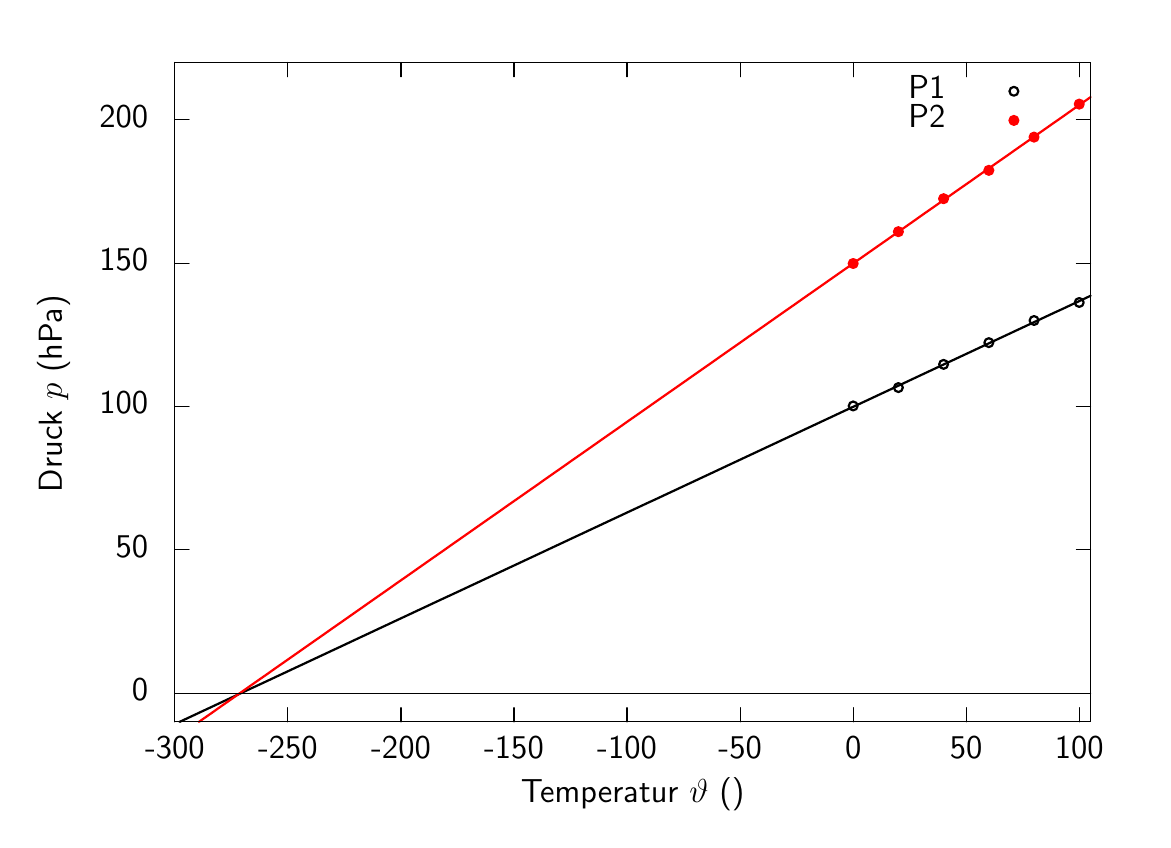
\begin{tikzpicture}[gnuplot]
%% generated with GNUPLOT 4.6p1 (Lua 5.1; terminal rev. 99, script rev. 100)
%% Mit 01 Mai 2013 11:47:56 CEST
\tikzset{every node/.append style={font={\sffamily\fontsize{12pt}{14.4pt}\selectfont}}}
\path (0.000,0.000) rectangle (14.100,10.000);
\gpcolor{color=gp lt color border}
\gpsetlinetype{gp lt border}
\gpsetlinewidth{1.00}
\draw[gp path] (1.806,1.548)--(1.986,1.548);
\draw[gp path] (13.436,1.548)--(13.256,1.548);
\node[gp node right] at (1.585,1.548) { 0};
\draw[gp path] (1.806,3.368)--(1.986,3.368);
\draw[gp path] (13.436,3.368)--(13.256,3.368);
\node[gp node right] at (1.585,3.368) { 50};
\draw[gp path] (1.806,5.188)--(1.986,5.188);
\draw[gp path] (13.436,5.188)--(13.256,5.188);
\node[gp node right] at (1.585,5.188) { 100};
\draw[gp path] (1.806,7.009)--(1.986,7.009);
\draw[gp path] (13.436,7.009)--(13.256,7.009);
\node[gp node right] at (1.585,7.009) { 150};
\draw[gp path] (1.806,8.829)--(1.986,8.829);
\draw[gp path] (13.436,8.829)--(13.256,8.829);
\node[gp node right] at (1.585,8.829) { 200};
\draw[gp path] (1.806,1.184)--(1.806,1.364);
\draw[gp path] (1.806,9.557)--(1.806,9.377);
\node[gp node center] at (1.806,0.814) {-300};
\draw[gp path] (3.242,1.184)--(3.242,1.364);
\draw[gp path] (3.242,9.557)--(3.242,9.377);
\node[gp node center] at (3.242,0.814) {-250};
\draw[gp path] (4.678,1.184)--(4.678,1.364);
\draw[gp path] (4.678,9.557)--(4.678,9.377);
\node[gp node center] at (4.678,0.814) {-200};
\draw[gp path] (6.113,1.184)--(6.113,1.364);
\draw[gp path] (6.113,9.557)--(6.113,9.377);
\node[gp node center] at (6.113,0.814) {-150};
\draw[gp path] (7.549,1.184)--(7.549,1.364);
\draw[gp path] (7.549,9.557)--(7.549,9.377);
\node[gp node center] at (7.549,0.814) {-100};
\draw[gp path] (8.985,1.184)--(8.985,1.364);
\draw[gp path] (8.985,9.557)--(8.985,9.377);
\node[gp node center] at (8.985,0.814) {-50};
\draw[gp path] (10.421,1.184)--(10.421,1.364);
\draw[gp path] (10.421,9.557)--(10.421,9.377);
\node[gp node center] at (10.421,0.814) { 0};
\draw[gp path] (11.857,1.184)--(11.857,1.364);
\draw[gp path] (11.857,9.557)--(11.857,9.377);
\node[gp node center] at (11.857,0.814) { 50};
\draw[gp path] (13.292,1.184)--(13.292,1.364);
\draw[gp path] (13.292,9.557)--(13.292,9.377);
\node[gp node center] at (13.292,0.814) { 100};
\draw[gp path] (1.806,9.557)--(1.806,1.184)--(13.436,1.184)--(13.436,9.557)--cycle;
\node[gp node center,rotate=-270] at (0.295,5.370) {Druck $p$ (hPa)};
\node[gp node center] at (7.621,0.259) {Temperatur $\vartheta$ (\SI{}{\celsius})};
\node[gp node right] at (11.709,9.192) {P1};
\gpcolor{rgb color={0.000,0.000,0.000}}
\gpsetlinewidth{2.00}
\gpsetpointsize{4.00}
\gppoint{gp mark 6}{(10.421,5.196)}
\gppoint{gp mark 6}{(10.995,5.429)}
\gppoint{gp mark 6}{(11.569,5.724)}
\gppoint{gp mark 6}{(12.144,6.000)}
\gppoint{gp mark 6}{(12.718,6.281)}
\gppoint{gp mark 6}{(13.292,6.510)}
\gppoint{gp mark 6}{(12.462,9.192)}
\gpsetlinetype{gp lt plot 0}
\draw[gp path] (1.868,1.184)--(1.923,1.210)--(2.041,1.265)--(2.158,1.320)--(2.276,1.375)%
  --(2.393,1.430)--(2.511,1.485)--(2.628,1.540)--(2.746,1.595)--(2.863,1.649)--(2.981,1.704)%
  --(3.098,1.759)--(3.216,1.814)--(3.333,1.869)--(3.451,1.924)--(3.568,1.979)--(3.686,2.034)%
  --(3.803,2.089)--(3.921,2.144)--(4.038,2.199)--(4.155,2.254)--(4.273,2.309)--(4.390,2.364)%
  --(4.508,2.419)--(4.625,2.474)--(4.743,2.529)--(4.860,2.584)--(4.978,2.639)--(5.095,2.694)%
  --(5.213,2.749)--(5.330,2.803)--(5.448,2.858)--(5.565,2.913)--(5.683,2.968)--(5.800,3.023)%
  --(5.918,3.078)--(6.035,3.133)--(6.153,3.188)--(6.270,3.243)--(6.388,3.298)--(6.505,3.353)%
  --(6.622,3.408)--(6.740,3.463)--(6.857,3.518)--(6.975,3.573)--(7.092,3.628)--(7.210,3.683)%
  --(7.327,3.738)--(7.445,3.793)--(7.562,3.848)--(7.680,3.903)--(7.797,3.958)--(7.915,4.012)%
  --(8.032,4.067)--(8.150,4.122)--(8.267,4.177)--(8.385,4.232)--(8.502,4.287)--(8.620,4.342)%
  --(8.737,4.397)--(8.854,4.452)--(8.972,4.507)--(9.089,4.562)--(9.207,4.617)--(9.324,4.672)%
  --(9.442,4.727)--(9.559,4.782)--(9.677,4.837)--(9.794,4.892)--(9.912,4.947)--(10.029,5.002)%
  --(10.147,5.057)--(10.264,5.112)--(10.382,5.167)--(10.499,5.221)--(10.617,5.276)--(10.734,5.331)%
  --(10.852,5.386)--(10.969,5.441)--(11.087,5.496)--(11.204,5.551)--(11.321,5.606)--(11.439,5.661)%
  --(11.556,5.716)--(11.674,5.771)--(11.791,5.826)--(11.909,5.881)--(12.026,5.936)--(12.144,5.991)%
  --(12.261,6.046)--(12.379,6.101)--(12.496,6.156)--(12.614,6.211)--(12.731,6.266)--(12.849,6.321)%
  --(12.966,6.376)--(13.084,6.430)--(13.201,6.485)--(13.319,6.540)--(13.436,6.595);
\gpcolor{color=gp lt color border}
\node[gp node right] at (11.709,8.822) {P2};
\gpcolor{rgb color={1.000,0.000,0.000}}
\gppoint{gp mark 7}{(10.421,7.005)}
\gppoint{gp mark 7}{(10.995,7.409)}
\gppoint{gp mark 7}{(11.569,7.828)}
\gppoint{gp mark 7}{(12.144,8.188)}
\gppoint{gp mark 7}{(12.718,8.610)}
\gppoint{gp mark 7}{(13.292,9.029)}
\gppoint{gp mark 7}{(12.462,8.822)}
\draw[gp path] (2.113,1.184)--(2.158,1.216)--(2.276,1.298)--(2.393,1.381)--(2.511,1.463)%
  --(2.628,1.545)--(2.746,1.628)--(2.863,1.710)--(2.981,1.792)--(3.098,1.875)--(3.216,1.957)%
  --(3.333,2.039)--(3.451,2.122)--(3.568,2.204)--(3.686,2.286)--(3.803,2.369)--(3.921,2.451)%
  --(4.038,2.533)--(4.155,2.615)--(4.273,2.698)--(4.390,2.780)--(4.508,2.862)--(4.625,2.945)%
  --(4.743,3.027)--(4.860,3.109)--(4.978,3.192)--(5.095,3.274)--(5.213,3.356)--(5.330,3.439)%
  --(5.448,3.521)--(5.565,3.603)--(5.683,3.686)--(5.800,3.768)--(5.918,3.850)--(6.035,3.933)%
  --(6.153,4.015)--(6.270,4.097)--(6.388,4.179)--(6.505,4.262)--(6.622,4.344)--(6.740,4.426)%
  --(6.857,4.509)--(6.975,4.591)--(7.092,4.673)--(7.210,4.756)--(7.327,4.838)--(7.445,4.920)%
  --(7.562,5.003)--(7.680,5.085)--(7.797,5.167)--(7.915,5.250)--(8.032,5.332)--(8.150,5.414)%
  --(8.267,5.496)--(8.385,5.579)--(8.502,5.661)--(8.620,5.743)--(8.737,5.826)--(8.854,5.908)%
  --(8.972,5.990)--(9.089,6.073)--(9.207,6.155)--(9.324,6.237)--(9.442,6.320)--(9.559,6.402)%
  --(9.677,6.484)--(9.794,6.567)--(9.912,6.649)--(10.029,6.731)--(10.147,6.814)--(10.264,6.896)%
  --(10.382,6.978)--(10.499,7.060)--(10.617,7.143)--(10.734,7.225)--(10.852,7.307)--(10.969,7.390)%
  --(11.087,7.472)--(11.204,7.554)--(11.321,7.637)--(11.439,7.719)--(11.556,7.801)--(11.674,7.884)%
  --(11.791,7.966)--(11.909,8.048)--(12.026,8.131)--(12.144,8.213)--(12.261,8.295)--(12.379,8.377)%
  --(12.496,8.460)--(12.614,8.542)--(12.731,8.624)--(12.849,8.707)--(12.966,8.789)--(13.084,8.871)%
  --(13.201,8.954)--(13.319,9.036)--(13.436,9.118);
\gpcolor{color=gp lt color border}
\gpsetlinetype{gp lt border}
\gpsetlinewidth{1.00}
\draw[gp path] (1.806,1.548)--(1.923,1.548)--(2.041,1.548)--(2.158,1.548)--(2.276,1.548)%
  --(2.393,1.548)--(2.511,1.548)--(2.628,1.548)--(2.746,1.548)--(2.863,1.548)--(2.981,1.548)%
  --(3.098,1.548)--(3.216,1.548)--(3.333,1.548)--(3.451,1.548)--(3.568,1.548)--(3.686,1.548)%
  --(3.803,1.548)--(3.921,1.548)--(4.038,1.548)--(4.155,1.548)--(4.273,1.548)--(4.390,1.548)%
  --(4.508,1.548)--(4.625,1.548)--(4.743,1.548)--(4.860,1.548)--(4.978,1.548)--(5.095,1.548)%
  --(5.213,1.548)--(5.330,1.548)--(5.448,1.548)--(5.565,1.548)--(5.683,1.548)--(5.800,1.548)%
  --(5.918,1.548)--(6.035,1.548)--(6.153,1.548)--(6.270,1.548)--(6.388,1.548)--(6.505,1.548)%
  --(6.622,1.548)--(6.740,1.548)--(6.857,1.548)--(6.975,1.548)--(7.092,1.548)--(7.210,1.548)%
  --(7.327,1.548)--(7.445,1.548)--(7.562,1.548)--(7.680,1.548)--(7.797,1.548)--(7.915,1.548)%
  --(8.032,1.548)--(8.150,1.548)--(8.267,1.548)--(8.385,1.548)--(8.502,1.548)--(8.620,1.548)%
  --(8.737,1.548)--(8.854,1.548)--(8.972,1.548)--(9.089,1.548)--(9.207,1.548)--(9.324,1.548)%
  --(9.442,1.548)--(9.559,1.548)--(9.677,1.548)--(9.794,1.548)--(9.912,1.548)--(10.029,1.548)%
  --(10.147,1.548)--(10.264,1.548)--(10.382,1.548)--(10.499,1.548)--(10.617,1.548)--(10.734,1.548)%
  --(10.852,1.548)--(10.969,1.548)--(11.087,1.548)--(11.204,1.548)--(11.321,1.548)--(11.439,1.548)%
  --(11.556,1.548)--(11.674,1.548)--(11.791,1.548)--(11.909,1.548)--(12.026,1.548)--(12.144,1.548)%
  --(12.261,1.548)--(12.379,1.548)--(12.496,1.548)--(12.614,1.548)--(12.731,1.548)--(12.849,1.548)%
  --(12.966,1.548)--(13.084,1.548)--(13.201,1.548)--(13.319,1.548)--(13.436,1.548);
\draw[gp path] (1.806,9.557)--(1.806,1.184)--(13.436,1.184)--(13.436,9.557)--cycle;
%% coordinates of the plot area
\gpdefrectangularnode{gp plot 1}{\pgfpoint{1.806cm}{1.184cm}}{\pgfpoint{13.436cm}{9.557cm}}
\end{tikzpicture}
%% gnuplot variables

\item [b)] Druck und Temperatur sind proportional.
\item [c)] Beim Druck von \SI{0}{Pa} sollten sich beide Kurven schneiden. Der Schnittpunkt ist bei Kurven ist im 
	Idealfall bei $\vartheta=\SI{-273.15}{\celsius}$. Das ist der absolute Nullpunkt der Temperatur. Dieser bekommt den Wert Null (\SI{0}{K}).
	Null Kelvin.
	\end{itemize}
\end{loesung}
\end{aufgabe}


\subsection{Gesetz von Boyle-Mariotte}
Im folgenden wollen wir untersuchen wie Druck und Volumen eines Gases miteinander zusammenhängen.
Dabei soll die Gasmenge, also die Anzahl von Gasatomen (Gasmolekülen) konstant sein.
Ausserdem wollen wir die Temperatur konstant halten.

\begin{aufgabe}
	\begin{itemize}
		\item Tragen Sie die Messwerte des Experiments in die Tabelle ein.
		\item Vervollständigen sie die letzten zwei Spalten. 
		\item Zeichnen Sie die Messpunkte des Experiments in ein $pV$-Diagramm ein.
		\item Was gilt für das Produkt von Druck und Volumen wenn die Gasmenge und die Temperatur konstant gehalten werden?
	\end{itemize}
	\begin{loesung}
		Das Produkt aus Druck und Temperatur ist konstant.
	\end{loesung}
\end{aufgabe}

\subsubsection*{Messwerte des Experiments}

\begin{center}
\begin{tabular}{p{3cm}|p{3cm}||p{3cm}|p{3cm}}
	\large{Druck} & \large{Kolbenstellung}  & \large{Volumen}  & $p\cdot V$\\\hline
	              &                         &                  & \\
	              &                         &                  & \\\hline
	              &                         &                  & \\
	              &                         &                  & \\\hline
	              &                         &                  & \\
	              &                         &                  & \\\hline
	              &                         &                  & \\
	              &                         &                  & \\\hline
	              &                         &                  & \\
	              &                         &                  & \\\hline
	              &                         &                  & \\
	              &                         &                  & \\\hline
	              &                         &                  & \\
	              &                         &                  & \\\hline
	              &                         &                  & \\
	              &                         &                  & \\\hline
\end{tabular}
\end{center}




\begin{aufgabe}
	Ein Gas bei Normaldruck (\SI{1013}{hPa}) füllt ein Volumen von \SI{1.5}{m^3}. Wie hoch ist der Druck,
	nachdem das Volumen auf \SI{1}{m^3} reduziert wurde?
	\begin{loesung}
		\begin{eqnarray*}
			p\cdot V = \text{konstant} \to p_1\cdot V_1 = p_2\cdot V_2 \to p_2 =\frac{V_1}{V_2}\cdot p_1=\frac{\SI{1.5}{m^3}}{\SI{1}{m^3}}\cdot \SI{101300}{Pa}=\SI{151950}{Pa}
		\end{eqnarray*}
	\end{loesung}
\end{aufgabe}

Durch die letzten zwei Experimente haben wir zwei Eigenschaften des idealen Gases kennengelernt.
Im ersten Teil haben wir gesehen, dass das Verhältnis von Druck und Temperatur konstant ist ($p/T =\text{konst.}$).
Das Gesetz von Boyle-Mariotte besagt, dass das Produkt von Druck und Volumen konstant ist ($p\cdot V =\text{konst.}$).

Diese zwei Zusammenhänge lassen sich durch einen ersetzten.
\begin{eqnarray*}
	\frac{p\cdot V}{T} = \text{konstant}
\end{eqnarray*}

\begin{aufgabe}
	Das Volumen eines Gases von \SI{5}{l} und einem Druck von \SI{1013}{hPa} wird durch Kompression halbiert. 
	Gleichzeitig wird das Gas von \SI{15}{\celsius} auf \SI{95}{\celsius} erwärmt. 
	Wie hoch ist der Enddruck?
	\begin{loesung}
		\begin{eqnarray*}
			\frac{p\cdot V}{T}=\text{konstant}\to \frac{p_1\cdot V_1}{T_1}=\frac{p_2\cdot V_2}{T_2}\to p_2 =\frac{V_1}{V_2}\cdot\frac{T_2}{T_1}\cdot p_1=\num{2}\cdot\frac{\SI{368}{K}}{\SI{288}{K}}\cdot\SI{101300}{Pa}=\SI{258880}{Pa}
		\end{eqnarray*}
	\end{loesung}
\end{aufgabe}

\begin{aufgabe}
	Der Gasdruck in einem Gasthermometer mit konstantem Volumen betrage \SI{0.4}{bar} am Gefrierpunkt
	und \SI{0.546}{bar} am Siedepunkt des Wassers.
	\begin{itemize}
		\item [a)] Bei welcher Temperatur beträgt der Druck \SI{0.1}{bar}?
		\item [b)] Wie hoch ist der Druck bei der Temperatur bei der Schwefel siedet? ($\vartheta=\SI{444.6}{\celsius}$)
	\end{itemize}
	\begin{loesung}
		\begin{itemize}
			\item [a)]
				\begin{eqnarray*}
					\frac{p\cdot V}{T}=\text{konstant}\to\frac{p_1\cdot V_1}{T_1}=\frac{p_2\cdot V_2}{T_2}\to T_2=\frac{p_2}{p_1}\cdot\frac{V_2}{V_1}\cdot T_1 =\frac{1}{4}\cdot 1\cdot \SI{273}{K}=\SI{68.25}{K} 
				\end{eqnarray*}
			\item[b)]
				\begin{eqnarray*}
					\frac{p\cdot V}{T}=\text{konstant}\to\frac{p_1\cdot V_1}{T_1}=\frac{p_2\cdot V_2}{T_2}\to p_2=\frac{V_1}{V_2}\cdot\frac{T_2}{T_1}\cdot p_1=1\cdot\frac{\SI{717.75}{K}}{\SI{273.15}{K}}\cdot\SI{400}{hPa}=\SI{1051.1}{hPa} 
				\end{eqnarray*}
		\end{itemize}
	\end{loesung}
\end{aufgabe}

%\newpage

\subsection{Gasdruck und Gasmasse}
In einem Experiment wird wird das Gewicht von \SI{1}{L} Neon bei \SI{0}{\celsius} und \SI{1013}{hPa} bestimmt.
Dann pumpt man Neonatome aus dem Gefäss und misst Druck und Gewicht.
Die folgende Tabelle zeigt die Messwerte des Experiments.

\begin{center}
\begin{tabular}{lcccc}
	Druck (hPa)      & 1013      & 750        & 500        & 250 \\
	Gewicht (g)      & \num{0.9} & \num{0.67} & \num{0.44} & \num{0.22} \\
\end{tabular}
\end{center}

\begin{aufgabe}
	\begin{itemize}
		\item Zeichnen Sie die Messwerte aus der Tabelle in ein $m-p$-Diagramm ein.
		\item Wie ändert sich die Masse mit dem Druck?
	\end{itemize}
	\begin{loesung}
	Masse und Druck des Gases sind bei konstantem Volumen proportional.	
	\end{loesung}

\end{aufgabe}

Das Gewicht des Gases ist proportional zur Anzahl der Atome in dem Gas.


Die Menge eines Gases, das aus $N$ Atomen oder Molekülen besteht, kann durch seine Masse $m$
oder durch seine Stoffmenge $n$ beschrieben werden.
Es gilt:
\begin{eqnarray*}
	n=\frac{N}{N_A}=\frac{m}{M}\text{,} 
\end{eqnarray*}
dabei ist $N_A=\SI{6.02E23}{Teilchen/mol}$ die Avogadro'sche Zahl und $M$ die molare Masse.

\begin{aufgabe}
	Die molare Masse von Sauerstoff O$_2$ beträgt ca.~\SI{32}{g/mol}.
	Wie viele Mol Sauerstoff sind dann in einem Kilogramm?
	\begin{loesung}
		\begin{eqnarray*}
		n=\frac{m}{M}=\frac{\SI{1000}{g}}{\SI{32}{g/mol}}=\SI{31.25}{mol}
		\end{eqnarray*}
	\end{loesung}
\end{aufgabe}


\subsection{Gasmasse und Gassorte}

In einem Experiment wird das Gewicht von verschiedenen Gasen bei konstantem Volumen von \SI{1}{l},
konstantem Druck von \SI{1}{bar} und konstanter Temperatur von \SI{22}{\celsius} gemessen.

Vervollständigen Sie die Tabelle.
\begin{center}
\begin{tabular}{lccc}
	Gassorte  & Masse $m$ (g) & Molare Masse $M$ (g/mol)  & Stoffmenge $n$ (mol)\\\hline
	H$_2$     & \num{0.082}   & &\\
	He        & \num{0.163}   & &\\
	N$_2$     & \num{1.143}   & &\\
	CO$_2$    & \num{1.795}   & &\\
	SF$_6$    & \num{5.958}   & &\\
\end{tabular}
\end{center}

\subsection{Zustandsgleichung idealer Gase}
Nun werden wir die drei Gasgesetze zu einem Zusammenfassen.

Wir haben gesehen, dass für ein ideales Gas die Beziehung
\begin{eqnarray*}
	\frac{p\cdot V}{T} = \text{konstant}
\end{eqnarray*}
gilt.

Ausserdem ist für ein ideales Gas Druck $p$ und Masse $m$ verknüpft:
\begin{eqnarray*}
	\frac{p}{m}=\text{konstant}\text{.}
\end{eqnarray*}

Im letzten Abschnitt haben wir gesehen, dass
\begin{eqnarray*}
	\frac{m}{M}= \text{konstant}
\end{eqnarray*}
ist.

Daraus können wir
\begin{eqnarray*}
	\frac{p\cdot V \cdot M}{T\cdot m} = \text{konstant} = R
\end{eqnarray*}
schreiben. 
Das gibt die Zustandsgleichung des idealen Gases
\begin{eqnarray*}
	p\cdot V=n\cdot R\cdot T\text{.}
\end{eqnarray*}
Die Formel enthält nun alle Zustandsgrössen eines Gases. Die Konstante nennen wir $R$.
Sie heisst auch Gaskonstante und hat den Wert $R=\SI{8.314}{J/mol K}$.
Die Gaskonstante $R$ ist das Produkt aus Boltzmann-Konstante $k_B$ und Avogadro-Zahl $N_A$. 

Alternativ kann man die Zustandsgleichung des idealen Gases auch mit der Boltzmann-Konstanten $k_B$ schreiben.
Es gilt:
\begin{eqnarray*}
	p\cdot V = N\cdot k_B\cdot T\text{.}
\end{eqnarray*}

Die Boltzmann-Konstante hat einen Wert von $k_B=\SI{1.3806504E-23}{J/K}$.

\begin{aufgabe}
	Welches Volumen nimmt \SI{1}{mol} eines Gases bei \SI{0}{\celsius} und \SI{1}{bar} ein?
	\begin{loesung}
		\begin{eqnarray*}
			p\cdot V=n\cdot R\cdot T \to V=\frac{n\cdot R\cdot T}{p}=\frac{\SI{1}{mol}\cdot\SI{8.314}{J/mol K}\cdot\SI{273}{K}}{\SI{100000}{Pa}}=\SI{0.022697}{m^3}=\SI{22.7}{l}
		\end{eqnarray*}
	\end{loesung}
\end{aufgabe}

\begin{aufgabe}
	\SI{1}{mol} eines Gases nimmt ein Volumen von \SI{10}{l} bei einem Druck von \SI{1}{bar} ein.
	Wie hoch ist seine Temperatur in Kelvin?
	\begin{loesung}
		\begin{eqnarray*}
			p\cdot V=n\cdot R\cdot T \to T=\frac{p\cdot V}{n\cdot R}=\frac{\SI{100000}{Pa}\cdot\SI{0.01}{m^3}}{\SI{1}{mol}\cdot\SI{8.314}{J/mol K}}=\frac{\SI{1000}{Pa m^3}}{\SI{8.314}{J/ K}}=\SI{120.28}{K}
		\end{eqnarray*}
	\end{loesung}
\end{aufgabe}

\begin{aufgabe}
	Eine bestimmte Gasmenge werde bei konstantem Druck gehalten. Um welchen Faktor ändert sich
	ihr Volumen, wenn die Temperatur von \SI{50}{\celsius} auf \SI{100}{\celsius} erhöht wird.
	\begin{loesung}
		\begin{eqnarray*}
			\frac{p\cdot V}{T}=\text{konstant}\to\frac{p_1\cdot V_1}{T_1}=\frac{p_2\cdot V_2}{T_2}\to\frac{V_2}{V_1}=\frac{p_1}{p_2}\cdot\frac{T_2}{T_1}=1\cdot\frac{\SI{373}{K}}{\SI{323}{K}}=\num{1.15}
		\end{eqnarray*}
	\end{loesung}

\end{aufgabe}

\begin{aufgabe}
	Wie viele Mol Neon sind in einem Volumen von \SI{1}{cm^3} bei einer Temperatur von \SI{0}{\celsius} und \SI{1}{bar}?
	Wie viele Atome Neon sind das?
	\begin{loesung}
		\begin{eqnarray*}
			p\cdot V=n\cdot R\cdot T \to n=\frac{p\cdot V}{R\cdot T}=\frac{\SI{1E5}{Pa}\cdot\SI{1E-6}{m^3}}{R\cdot\SI{273}{K}}=\frac{\SI{1E-1}{Pa m^3}}{\SI{2269.7}{J/mol}}=\SI{4.4058e-5}{mol}
		\end{eqnarray*}
		\begin{eqnarray*}
			n=\frac{N}{N_A}\to N=n\cdot N_A=\SI{4.4058e-5}{mol}\cdot\SI{6.02E23}{1/mol}=\num{2.6523e+19}
		\end{eqnarray*}
	\end{loesung}
\end{aufgabe}




\newpage
\includesolutions


\end{document}
